\begin{frame}[noframenumbering,plain]
    \setcounter{framenumber}{1}
    \maketitle
\end{frame}

\section{Содержание}

\begin{frame}{Содержание}
	\LARGE
	\begin{enumerate}
		\item Введение
		\item Математические модели
		\item Численный алгоритм решения
		\item Программный комплекс NonLocFEM
		\item Анализ решений
		\item Заключение
	\end{enumerate}
    %\tableofcontents
\end{frame}

\section{Введение}
\begin{frame}
	\centering
	\Huge
	Введение
\end{frame}

\begin{frame}{Введение}
\begin{center}
	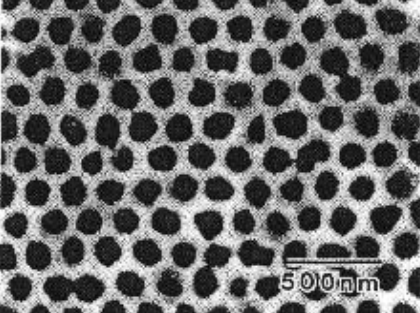
\includegraphics[width=0.27\linewidth]{pics/Al.png}
	\hfill
	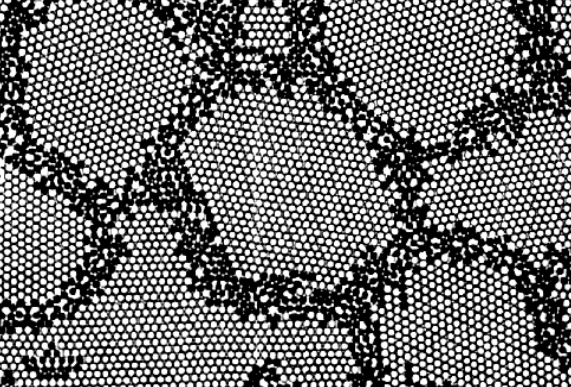
\includegraphics[width=0.3\linewidth]{pics/Atoms.png}
	\hfill
	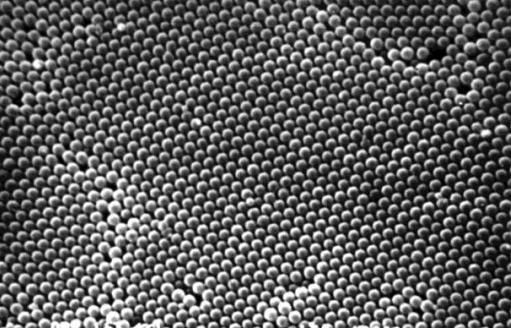
\includegraphics[width=0.32\linewidth]{pics/Kremnezem.png}
	
	Атомная решётка структурно-чувствительных материалов
\end{center}
\end{frame}

\begin{frame}
	\begin{center}
	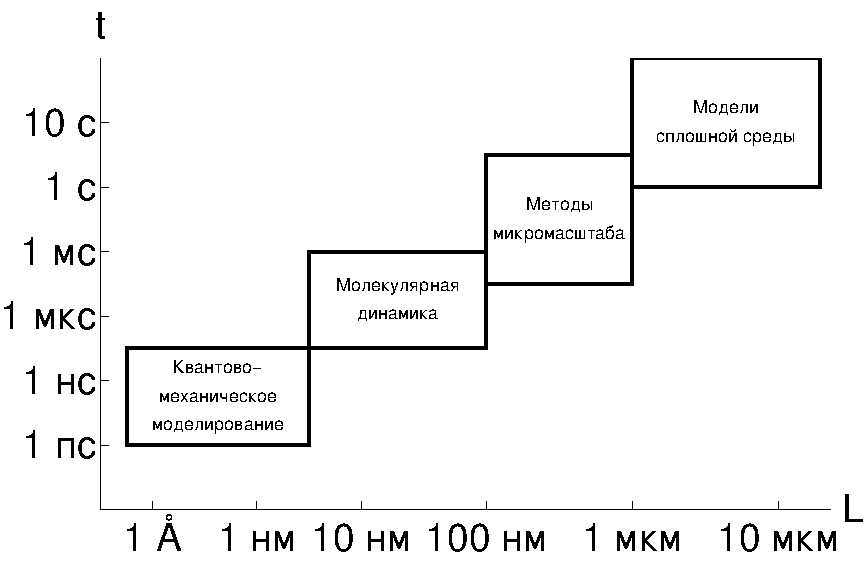
\includegraphics[width=0.85\textwidth]{pics/ModelsHierarchy.pdf}
	
	Иерархия моделей моделей механики твёрдого тела
	\end{center}
\end{frame}

\begin{frame}{Модели обобщённой механики сплошной среды}
	Модели сплошной среды, учитывающие структуру материала:
	\begin{itemize}
		\item \textbf{моментные модели}:
		\begin{itemize}
			\justifying
			\item \textbf{микрополярные} (Eugène и François Cosserat, V.~G{\"u}nther, Э.Л.~Аэро, Е.В.~Кувшинский, Никабадзе~М.У. и др.);
			\item \textbf{микроморфные} (A.C.~Eringen и др.);
		\end{itemize}
		\item \textbf{дальнодействующие эффекты}:
		\begin{itemize}
			\justifying
			\item \textbf{градиентные} (R.A.~Toupin, R.D.~Mindlin, E.C.~Aifantis, С.А.~Лурье, В.В.~Васильев и др.);
			\item \textbf{нелокальные} (E.~Kr{\"o}ner, A.C.~Eringen, D.~Rogula, D.G.B.~Edelen, S.B.~Altan, Г.Н.~Кувыркин, В.С.~Зарубин, И.Ю.~Савельева и др.);
		\end{itemize}
	\end{itemize}
\end{frame}

\begin{frame}
    \frametitle{Положения, выносимые на защиту}
    \begin{itemize}
    	\justifying
        \item Модели нелокальной теплопроводности и термоупругости, позволяющие описать процессы передачи теплоты и напряжённо-деформированного состояния в структурно-чувствительных материалах.
        \item Новые численные алгоритмы решения на основе метода конечных элементов, адапатированные под многопроцессорные вычислительные системы.
        \item Собственный программный комплекс NonLocFEM, в рамках которого реализованы все рассматриваемые в работе методы решений.
    \end{itemize}
\end{frame}
\note{
    Проговариваются вслух положения, выносимые на защиту
}
